\documentclass{report}
\usepackage[T1]{fontenc}
\usepackage{color}
\usepackage{amssymb}
\usepackage{pdfpages}
\usepackage{amsmath}
\usepackage{eurosym}
\usepackage{graphicx}
\usepackage{textcomp}
\usepackage{listings}
\usepackage{epigraph}
\usepackage{setspace}
\usepackage{array}
\usepackage{gensymb}
\usepackage{tikz}
\usepackage[some]{background}
\usepackage{geometry}
\usepackage[francais]{babel}


\begin{document}
\renewcommand{\contentsname}{Sommaire}
\renewcommand{\chaptername}{Partie}
\renewcommand{\thechapter}{\Roman{chapter}}

%\usepackage{lmodern}
%\usepackage{xspace}
%\usepackage{hyperref}

\definecolor{sup_strip_color}{rgb}{0.70,0.70,0.70}
\definecolor{inf_strip_color}{rgb}{0.00,0.00,0.00}

\DeclareFixedFont{\bigsf}{T1}{phv}{b}{n}{0.7cm}

\makeatletter                       
\def\printauthor{%                  
    {{\large \@author}}}              
\makeatother

\author{Zohour \textsc{Abouakil} ~\\ Sofia \textsc{Boutahar} ~\\ David \textsc{Courtinot} ~\\ Xiaowen \textsc{Ji} ~\\ Fabien \textsc{Sauce}}

\begin{titlepage}

\newgeometry{left=1cm,right=4cm}
\begin{tikzpicture}[overlay,remember picture]
% the black stripe with the title
\node[
  fill=inf_strip_color,
  anchor=north west,
  text width=\paperwidth,
  text height=2cm,
  text depth=2cm,
  inner xsep=1cm,
  font=\color{white}\bigsf 
  ] 
 at ([yshift=-2.5cm]current page.north west) (blackrect) {Plan de d\'{e}veloppement};
% the khaki stripe
\path[fill=sup_strip_color] 
  (blackrect.north west) rectangle ++(\paperwidth,2.5cm);
\end{tikzpicture}

\vspace*{4.5cm}

\noindent
\begin{minipage}{0.35\linewidth}
    \begin{flushright}
        \printauthor
    \end{flushright}
\end{minipage} \hspace{15pt}
%
\begin{minipage}{0.02\linewidth}
    \rule{1pt}{175pt}
\end{minipage} \hspace{-10pt}
%
\begin{minipage}{0.6\linewidth}
\vspace{5pt}
\newenvironment{test}{\begin{center}}{\end{center}}
\hspace{10pt}
\begin{minipage}{\linewidth} 
Recherche de motifs dans un code C++ \`{a} l'aide de la logique temporelle
\end{minipage}
\end{minipage}

\end{titlepage}
\restoregeometry
\tableofcontents
\chapter{Description du projet et objectifs}

\section{Attentes du client}

\paragraph{}
\hspace{4mm}\textnormal{Le client attend une conception d'un prototype permettant la recherche de motifs dans un code
 C++ afin d'assurer certaines propri\'{e}t\'{e}s sur le code v\'{e}rifiabes par sa syntaxe.
 Pour cela, diff\'{e}rentes analyses seront mises en \oe{}uvre pour \'{e}viter les dysfonctionnements.
 Une partie de ces analyses consiste \`{a} \'{e}tudier le code embarqu\'{e} et \`{a} prouver que le code fait bien
 ce qu'il est cens\'{e} faire. D'autres analyses consistent \`{a} montrer que le code embarqu\'{e} respecte un
 certain nombre de r\`{e}gles de programmation. L'analyse consiste donc \`{a} rechercher ces motifs dans
 le code source.}

\paragraph{}
\hspace{4mm}\textnormal{Nous utiliserons pour ce faire la repr\'{e}sentation interne du code de Clang afin de construire des graphes que nous pourrons utilise r\`{a} l'aide de la logique temporelle.
Ce travail se d\'{e}compose donc en deux parties : le model checking (algorithmes de recherche etc) et les \'{e}tapes de transformation du code vers sa repr\'{e}sentation en graphe de flot de contr\^{o}le (GFC). 
Ces deux parties doivent fonctionner aussi bien de fa\c{c}on ind\'{e}pendante que l'une avec l'autre. La cha\^{i}ne de transformations et de traitements est pr\'{e}sent\'{e}e
dans la figure ci-dessous :}

\begin{center}
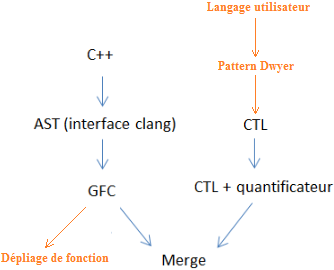
\includegraphics[scale=0.7]{data/tasks.png}
~\\~\\Figure I.1 - Cha\^{i}ne de transformations et de traitements
\end{center}

\section{Livrables et priorit\'{e}s}

\paragraph{}
\hspace{4mm}\textnormal{Les livrables attendu (et donc prioritaires) sont les suivants :}

\vspace{4mm}
\begin{itemize}
\item impl\'{e}mentation d'un parser pour l'AST produit par Clang\vspace{1mm}
\item une conversion AST vers un mod\`{e}le Scala de repr\'{e}sentation du code en termes de graphe de fulx de contr\^{o}le\vspace{1mm}
\item de fa\c{c}on ind\'{e}pendante des deux items pr\'{e}c\'{e}dents, des algorithmes d'analyse de propri\'{e}t\'{e}s de la logique temporelle sur des graphes de flux de contr\^{o}le
quelconques\vspace{1mm}
\item l'ajout \`{a} l'item pr\'{e}c\'{e}dent des quantificateurs tels que "il existe"\vspace{1mm}
\end{itemize}

\paragraph{}
\hspace{4mm}\textnormal{Les extensions suivantes pourront \^{e}tre ajout\'{e}es :}

\vspace{4mm}
\begin{itemize}
\item d\'{e}pliage des appels de fonctions sur une profondeur donn\'{e}e\vspace{1mm}
\item cr\'{e}ation d'un langage utilisateur servant d'interface avec le syst\`{e}me\vspace{1mm}
\end{itemize}

\chapter{Principes d'organisation}

\section{D\'{e}finition des r\^{o}les}

\subsubsection{Chef de projet}

\paragraph{}
\hspace{4mm}\textnormal{Le chef de projet s'occupe essentiellement des \'{e}changes et communications avec l'industriel et les clients. 
Il a un r\^{o}le pr\'{e}pond\'{e}rant dans l'organisation statique des t\^{a}ches.}

\subsubsection{Superviseur}

\paragraph{}
\hspace{4mm}\textnormal{Le superviseur a une vue globale du projet sur le plan technique. Il s'assure de l'avancement des t\^{a}ches simultan\'{e}es
et peut r\'{e}organiser les effectifs et les objectifs de fa\c{c}on dynamique dans le cas d'un impr\'{e}vu.
Le superviseur peut participer \`{a} l'\'{e}criture du code ou de la documentation mais il ne s'agit
pas de sa fonction premi\`{e}re. Pour finir, il peut varier d'une semaine sur l'autre.}

\subsubsection{Responsable qualit\'{e}}

\paragraph{}
\hspace{4mm}\textnormal{Le responsable qualit\'{e} d\'{e}finit des r\`{e}gles de bonne programmation et s'assure qu'elles sont v\'{e}rifi\'{e}es par les d\'{e}veloppeurs.
Tout code produit passera sous l'oeil attentif du responsable qualit\'{e} avant d'\^{e}tre valid\'{e}. Il assure \'{e}galement
la qualit\'{e} et la coh\'{e}rence de tous les documents produits par l'\'{e}quipe. Il est le seul \`{a} pouvoir pousser
du contenu sur le d\'{e}p\^{o}t Github, ou \`{a} autoriser un member un pousser.}

\subsubsection{Responsable de la validation et des tests}

\paragraph{}
\hspace{4mm}\textnormal{Le responsable de la validation est en charge des tests de validation en environnement global \'{e}crits par les programmeurs (chaque programmeur a son propre jeu de tests unitaires). Il ne se contente pas de les ex\'{e}cuter,
il d\'{e}termine \'{e}galement si ces tests sont suffisamment exhaustifs ou non.}

\section{Cha\^{i}ne de d\'{e}veloppement}

\subsection{Gestion de la qualit\'{e}}

\paragraph{}
\hspace{4mm}\textnormal{Avant d'\^{e}tre soumis \`{a} la validation, tout code produit passe par le responsable qualit\'{e}. Celui-ci \'{e}met, si besoin,
des recommandations d'am\'{e}lioration au programmeur. Le cas \'{e}ch\'{e}ant, le programmeur doit fournir une nouvelle version tenant compte
des remarques ou d\'{e}fendre ses choix s'il ne souhaite pas modifier son code. Ce va-et-vient se poursuit jusqu'\`{a} un consensus entre le programmeur
et le responsable qualit\'{e}.}

\subsection{Strat\'{e}gie de tests}

\paragraph{}
\hspace{4mm}\textnormal{Une fois la qualit\'{e} du code v\'{e}rifi\'{e}e, il est transmis au validateur qui lance les tests, v\'{e}rifie leur exhaustivit\'{e} et les compl\`{e}te si besoin.
Il n'est pas responsable du d\'{e}bugage du code, tout code \'{e}chouant aux tests est renvoy\'{e} \`{a} la personne les ayant d\'{e}velopp\'{e} avec un log d\'{e}taillant les tests en \'{e}chec.}

\subsection{Gestion de configuration}

\paragraph{}
\hspace{4mm}\textnormal{Une fois les deux \'{e}tapes pr\'{e}c\'{e}dentes achev\'{e}es, le validateur effectue ou autorise le d\'{e}p\^{o}t des sources concern\'{e}es
sur le gestionnaire de version. Le sch\'{e}ma global de cette organisation est donc le suivant :}

\begin{center}
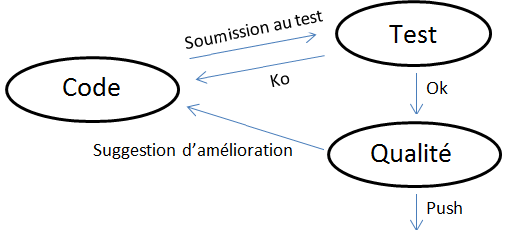
\includegraphics[scale=0.7]{data/cycle_qualite}
~\\~\\Figure II.1 - Sch\'{e}ma descriptif de la cha\^{i}ne de d\'{e}veloppement
\end{center}

\chapter{Planification}

\section{M\'{e}thode de d\'{e}veloppement et de programmation}

\subsection{Scrum}

\paragraph{}
\hspace{4mm}\textnormal{Nous nous efforcerons d'appliquer la m\'{e}thode Scrum, tr\`{e}s utilis\'{e}e actuellement et reconnue pour son efficacit\'{e}.
En somme, nous d\'{e}finissons tout d'abord un \textit{product backlog}, d\'{e}finissant tous les livrables du produit final. Le pr\'{e}sent
document fait office de \textit{backlog}. Par la suite, nous diviserons le projet en trois \textit{sprints} (ou \textit{it\'{e}rations}).
Pour chacun d'entre eux, nous d\'{e}finirons le \textit{sprint backlog}, r\'{e}sumant tous les objectifs \`{a} atteindre
\`{a} l'issue de cette it\'{e}ration.
Chaque \textit{sprint} s'\'{e}tendra sur une p\'{e}riode de deux semaines et consistera \`{a} am\'{e}liorer le logiciel
de fa\c{c}on incr\'{e}mentale en y int\'{e}grant un \'{e}l\'{e}ment du \textit{product backlog}.}

\paragraph{}
\hspace{4mm}\textnormal{Apr\`{e}s chaque sprint, nous tiendrons une r\'{e}union pour faire un bilan de l'avancement, et proposer des am\'{e}liorations ou rectifications de trajectoire
(au cours d'une it\'{e}ration, la d\'{e}finition du \textit{sprint backlog} ne peut \^{e}tre modifi\'{e}e).
Enfin, chaque journ\'{e}e d\'{e}butera par un \textit{scrum meeting} o\`{u} chacun pr\'{e}sentera son travail de la veille
et exposera ses objectifs pour la journ\'{e}e ainsi que les \'{e}ventuelles difficult\'{e}s qu'il traverse actuellement.}

\subsection{R\'{e}partition du travail d'impl\'{e}mentation}

\paragraph{}
\hspace{4mm}\textnormal{Nous utiliserons une approche s'inspirant de la m\'{e}thode XP. En effet, nous jugeons que l'ampleur du projet ne n\'{e}cessite pas
que chaque membre du groupe programme s\'{e}par\'{e}ment, et nous estimons que la programmation en bin\^{o}me est un excellent
moyen de pr\'{e}venir les erreurs en amont et gagner beaucoup de temps en tests et d\'{e}bugage. Nous programmerons donc par bin\^{o}me, et le cinqui\`{e}me du groupe
d\'{e}veloppera seul. La composition des groupes pourra varier \`{a} mesure que les t\^{a}ches sont remplies.}

\section{D\'{e}composition en t\^{a}ches}

\section{Planning}

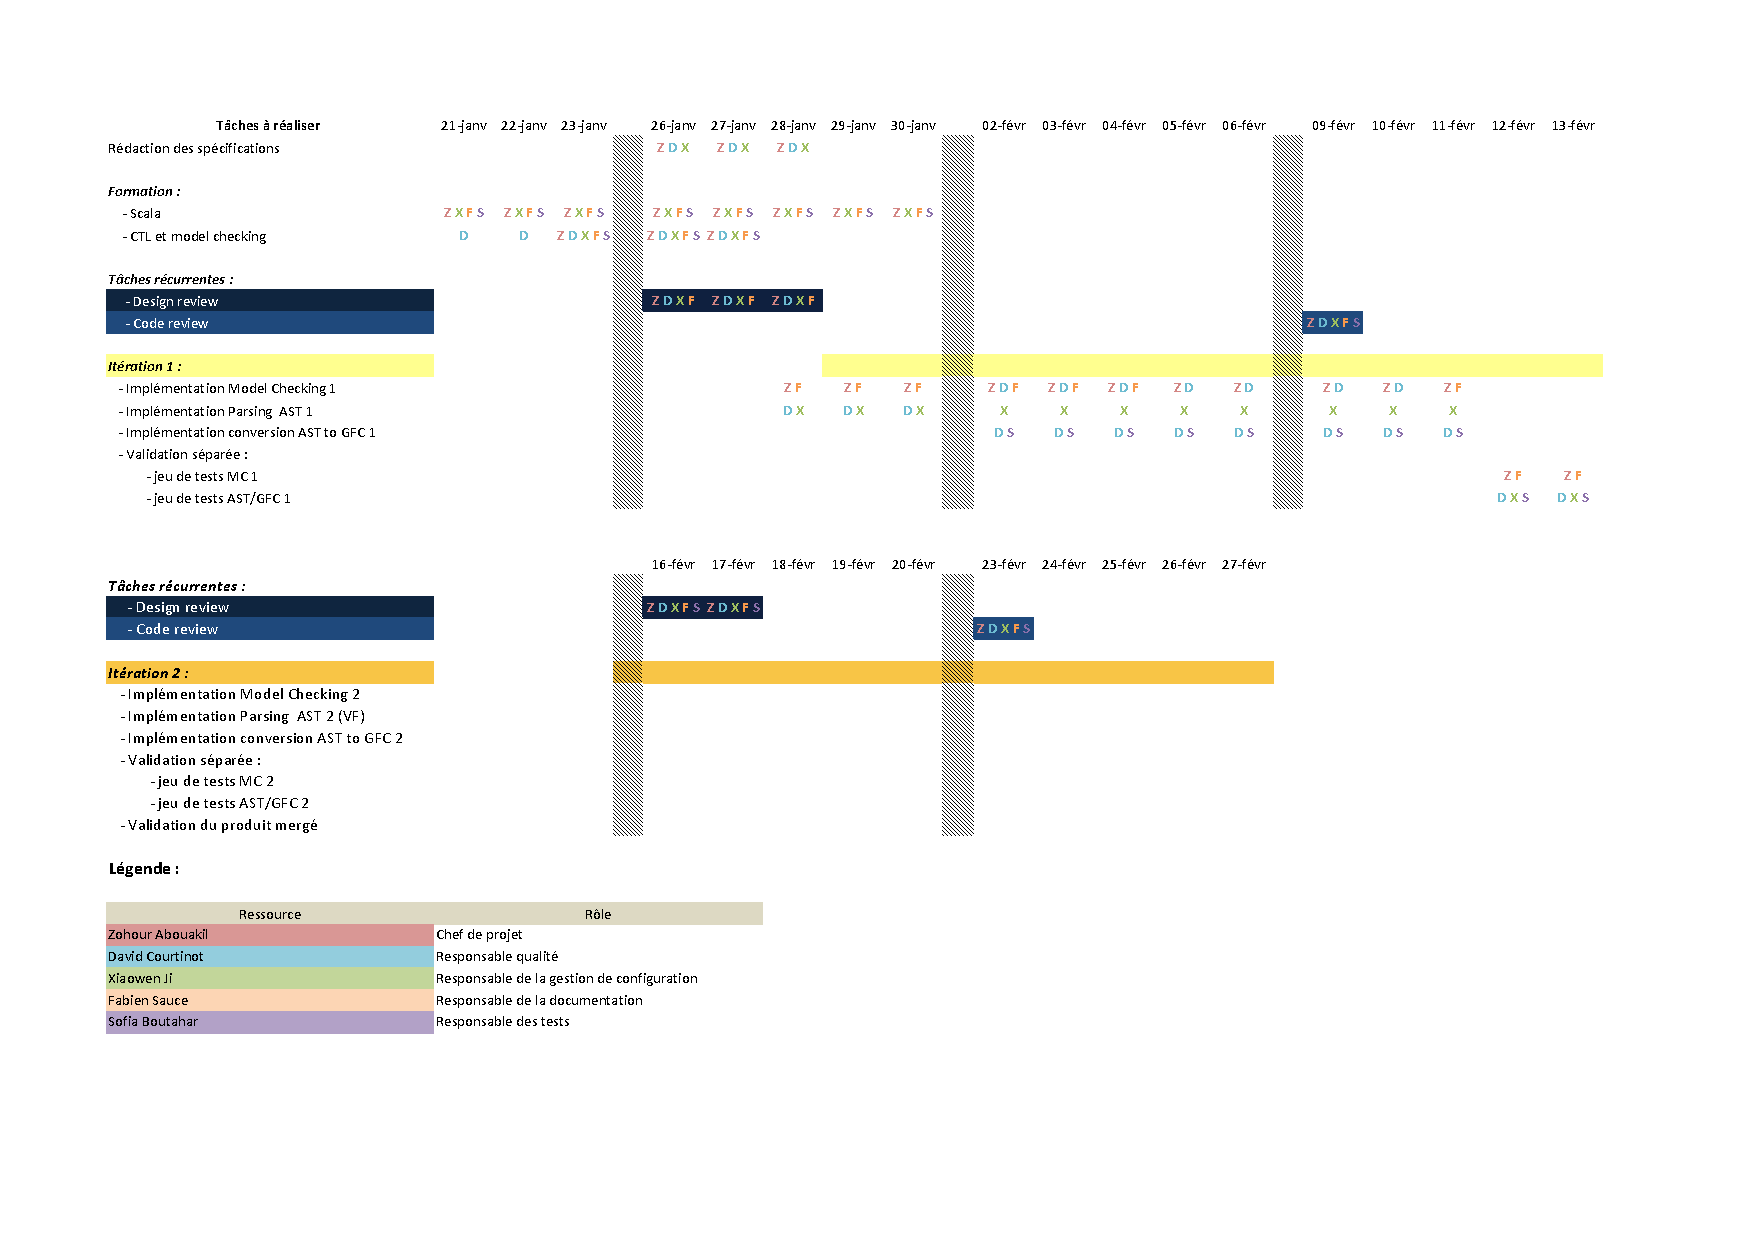
\includepdf[landscape=true,pages={1-2}]{data/planning.pdf}
\chapter{Gestion des risques}

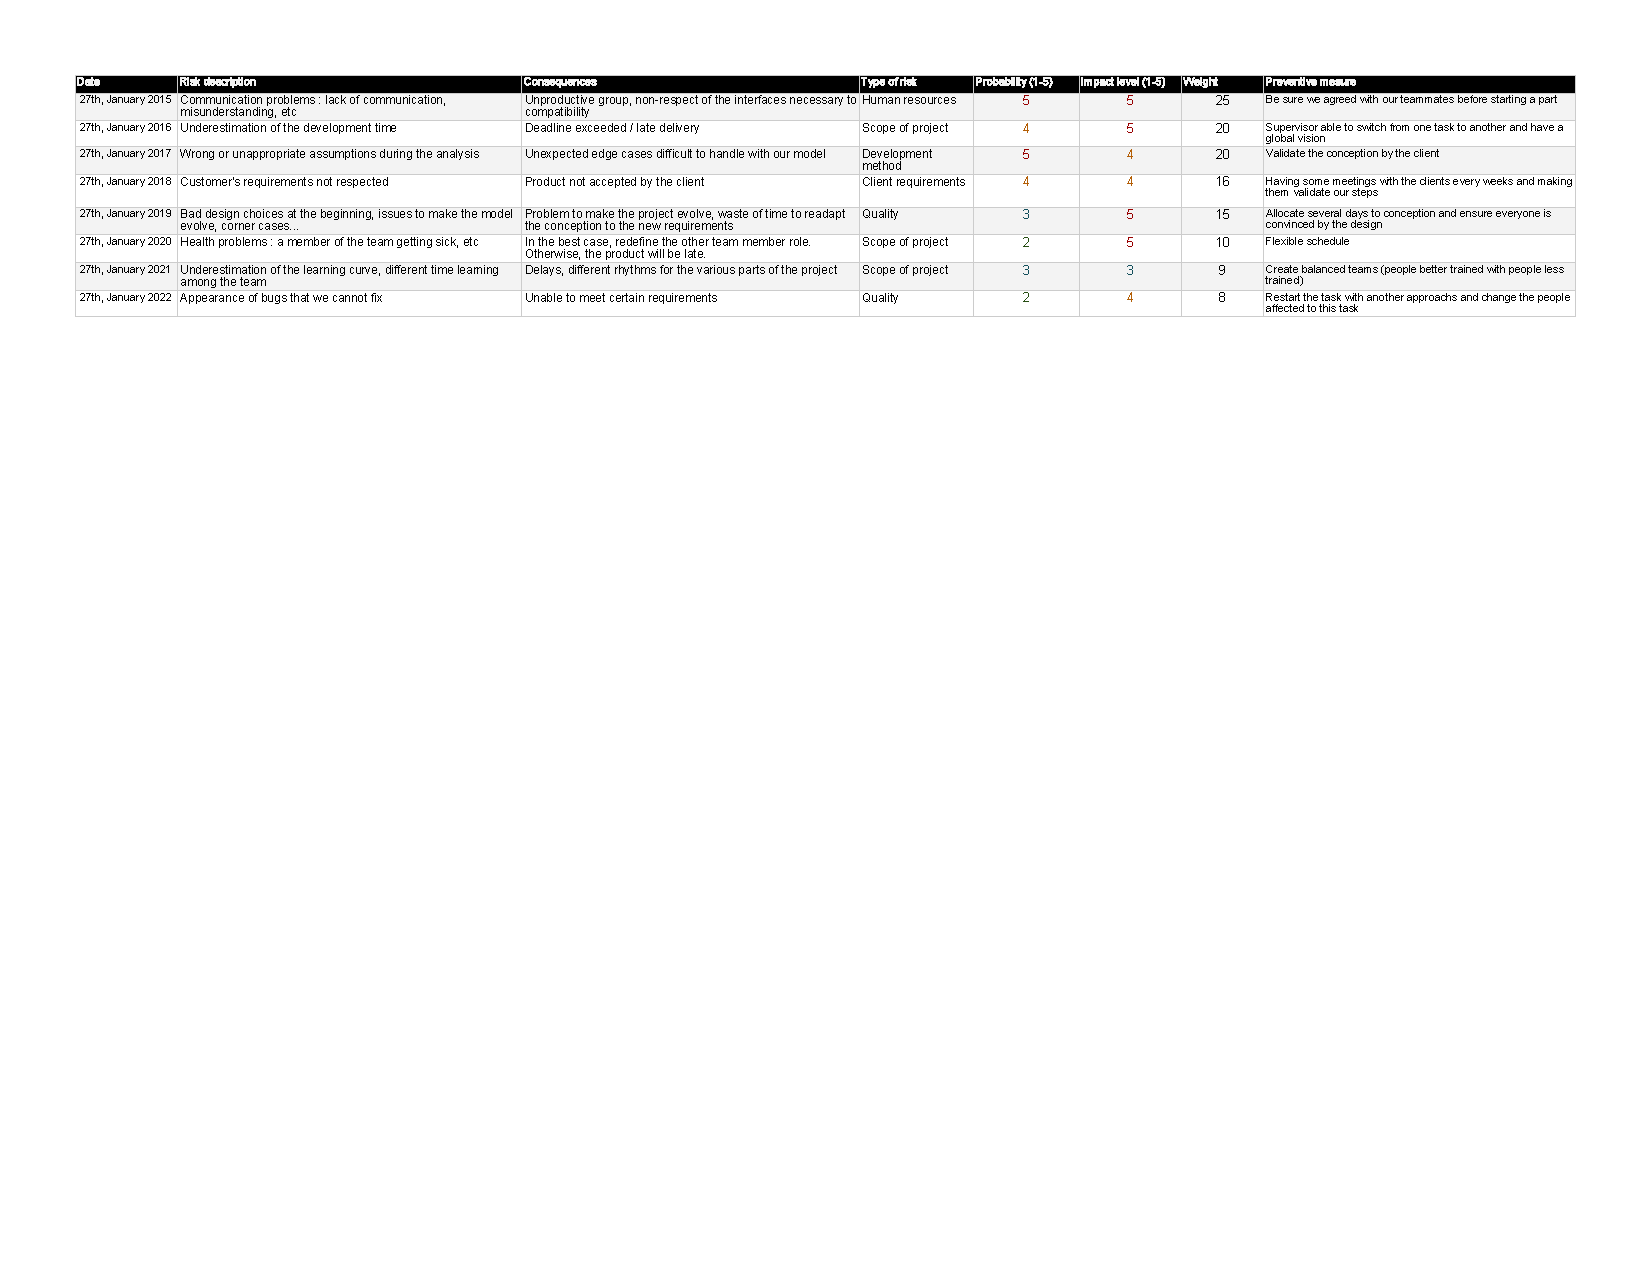
\includepdf[landscape=true,pages={1}]{data/risks.pdf}
\end{document}
